%%%%%%%%%%%%%%%%%%%%%%%%%%%%%%%%%%%%%%%%%%%%%%%%%%%%%%%%%%%%%%%%%%%%%%%%%%%%%%%
% Titel:   Abstract
% Autor:   S. Grossenbacher
% Datum:   27.09.2013
% Version: 1.0.0
%%%%%%%%%%%%%%%%%%%%%%%%%%%%%%%%%%%%%%%%%%%%%%%%%%%%%%%%%%%%%%%%%%%%%%%%%%%%%%%

%:::Change-Log:::
% Versionierung erfolgt auf folgende Gegebenheiten: -1. Stelle Semester
%                                                   -2. Stelle neuer Inhalt
%                                                   -3. Fehlerkorrekturen
%
% 1.0.0       Erstellung der Datei

%%%%%%%%%%%%%%%%%%%%%%%%%%%%%%%%%%%%%%%%%%%%%%%%%%%%%%%%%%%%%%%%%%%%%%%%%%%%%%%
\chapter*{Abstract}\todo{Elektroteil}
	Als \gls{ac:kernteam} besteht eine unserer Hauptaufgaben darin die vier Subteams zu koordinieren. Ganz zu Beginn der \gls{ac:pa2} muss in diesem Aufgabenbereich gehandelt werden. Nach Abschluss der \gls{ac:pa1} sind die Zielsetzungen des Subteams Antrieb nicht zufriedenstellend erreicht worden. Damit in der \gls{ac:pa2} die Defizite aufgeholt werden k�nnen ist eine personelle Umstrukturierung zwingend n�tig. Das Antriebsteam wird komplett neu gebildet. Zus�tzlich sind freigeworden personell Ressourcen in Subteams untergebracht worden, welche diese in der \gls{ac:pa2} ben�tigen. Das \gls{g:eurobot}-Team besteht in der \gls{ac:pa2} noch aus 11 Studenten.
	\par
	Die \gls{ac:pa2} befasst sich ansonsten prim�r mit dem Bereinigen der Mechanik im ersten Roboter und dem Erstellen des zweiten Roboters mit den Aufgaben \gls{g:fire} und \gls{g:mammut_catch} (Funny Action). Dazu kommt die Inbetriebnahme der beiden Roboter sowie das Testen der fertigen Teil- und Gesamtsysteme.
	\par 
	Konstruktive �nderungen m�ssen vor allem am Speerspick-Mechanismus vorgenommen werden. Erste Funktionstests des Systems zeigten, dass eine Vereinzelung der Speere unumg�nglich ist. Dazu kommen weitere kleine �nderungen im Bereich des Antriebs und des Linearmoduls der Bilderaufgabe. 
	Bei der Entwicklung der Handlingsysteme des zweiten Roboters wird vor allem die Umsetzung der Netzaufgabe in den Vordergrund gestellt. Dazu werden verschiedene Testaufbauten gebaut und getestet. Der Entscheid f�llt schlussendlich auf ein Wurfmechanismus �hnlich einer Armbrust, jedoch sind die Spannelemente am Netz befestigt. F�r die Feueraufgabe werden w�hrend der Konzeptphase keine Tests durchgef�hrt. Der Entscheid f�llt auf ein Hebelsystem welches �ber einen Vakuumsauger Feuer anheben und transportieren, jedoch nicht wenden kann.
	\par
	In der Ausarbeitungsphase stellten sich die Ausl�sung des Netzes f�r die \gls{g:mammut_catch}-Aufgabe, sowie das Netz selbst als grosse Herausforderung heraus. Schlussendlich wird ein Ausl�semechanismus konstruiert, welcher �ber ein Servo ausgel�st, jedoch ohne Servobet�tigung geladen werden kann. Es werden verschiedene Netze mit unterschiedlichen Steifigkeiten und Maschengr�ssen getestet. Die Wahl des Netzes f�llt schliesslich auf ein handels�bliches Feumernetz, das noch modifiziert wird. Die Feueraufgabe ist �ber ein Vakuumsaugsystem gel�st. Dabei kann der Vakuumsauger vertikal bewegt werden. Die Bewegung wird �ber ein Servo generiert.
	\par
	Vom Elektrotechnischen Aspekt her betrachtet, wurde erfolgreich eine Bedieneinheit mit einem kleinen Display und einigen Tastern umgesetzt, damit Initialisierungen wie zum Beispiel die Teamfarbe (Rot oder Gelb) eingestellt werden k�nnen.\\
	Ein weiterer Aufgabenbereich ist die Inbetriebnahme und Konfiguration s�mtlicher Ansteuerelemente (vor allem Servos) zum L�sen der Aufgaben. Dazu kommt das allgemeine Testen und Optimieren des Verhaltens des Roboter beim L�sen der Aufgaben.
	\par
	Damit die Roboter w�hrend einer Spielrunde auch ihn unvorhersehbaren Situationen angemessen handeln k�nnen, wurde das Augenmerk auf eine ausgefeilte Strategie gesetzt. Dabei soll unter der Beachtung von der Spielzeit, der Gegnerposition, der Distanz, usw... m�glichst viele Punkte gesammelt werden k�nnen. Umgesetzt hat man dies mit einer Kombination von g�ngigen Robotnik-Algorithmen. Dabei handelt es sich um den \textit{A-Star}-Algorithmus und dem \textit{Problem des Handelsreisenden}.\\
	Die Entwicklung der Strategie konnte so weit realisiert werden. Die Umsetzung und der Feinschliff ist jedoch noch in vollem Gange und wird auch noch bis kurz vor dem Turnier Arbeitszeit fordern.
	\par
	�ber das ganze Eurobotteam gesehen werden die Zielsetzungen der \gls{ac:pa2} gut erreicht. Die Probleme mit dem Antrieb haben sich aber weit in die \gls{ac:pa2} hineingezogen, was zu Verz�gerungen f�r das ganze \gls{g:eurobot}-Team f�hrte. So konnte bis zum Stand der Dokumentation noch nicht beide Roboter in Betrieb genommen werden, was jegliche Tests des Gesamtsystems verunm�glicht. 
	
	%Jedoch konnten bereits die Aufgaben \gls{g:fresko} und \gls{g:mammut} gel�st werden.
	
%	\par
%	Die beiden Roboter sind in den Abbildungen \ref{abb:robo_gross} und \ref{abb:robo_klein} zu sehen.
	%
%	\image{}{scale=1}{htbp}[Grosse Roboter ("B52")][abb:robo_gross]
%	%
%	\image{}{scale=1}{htbp}[Kleine Roboter ("Ballerina")][abb:robo_klein]

	\begin{figure}[htbp] %htbp
		\centering
		\begin{subfigure}[b]{0.49\textwidth}
			\centering
			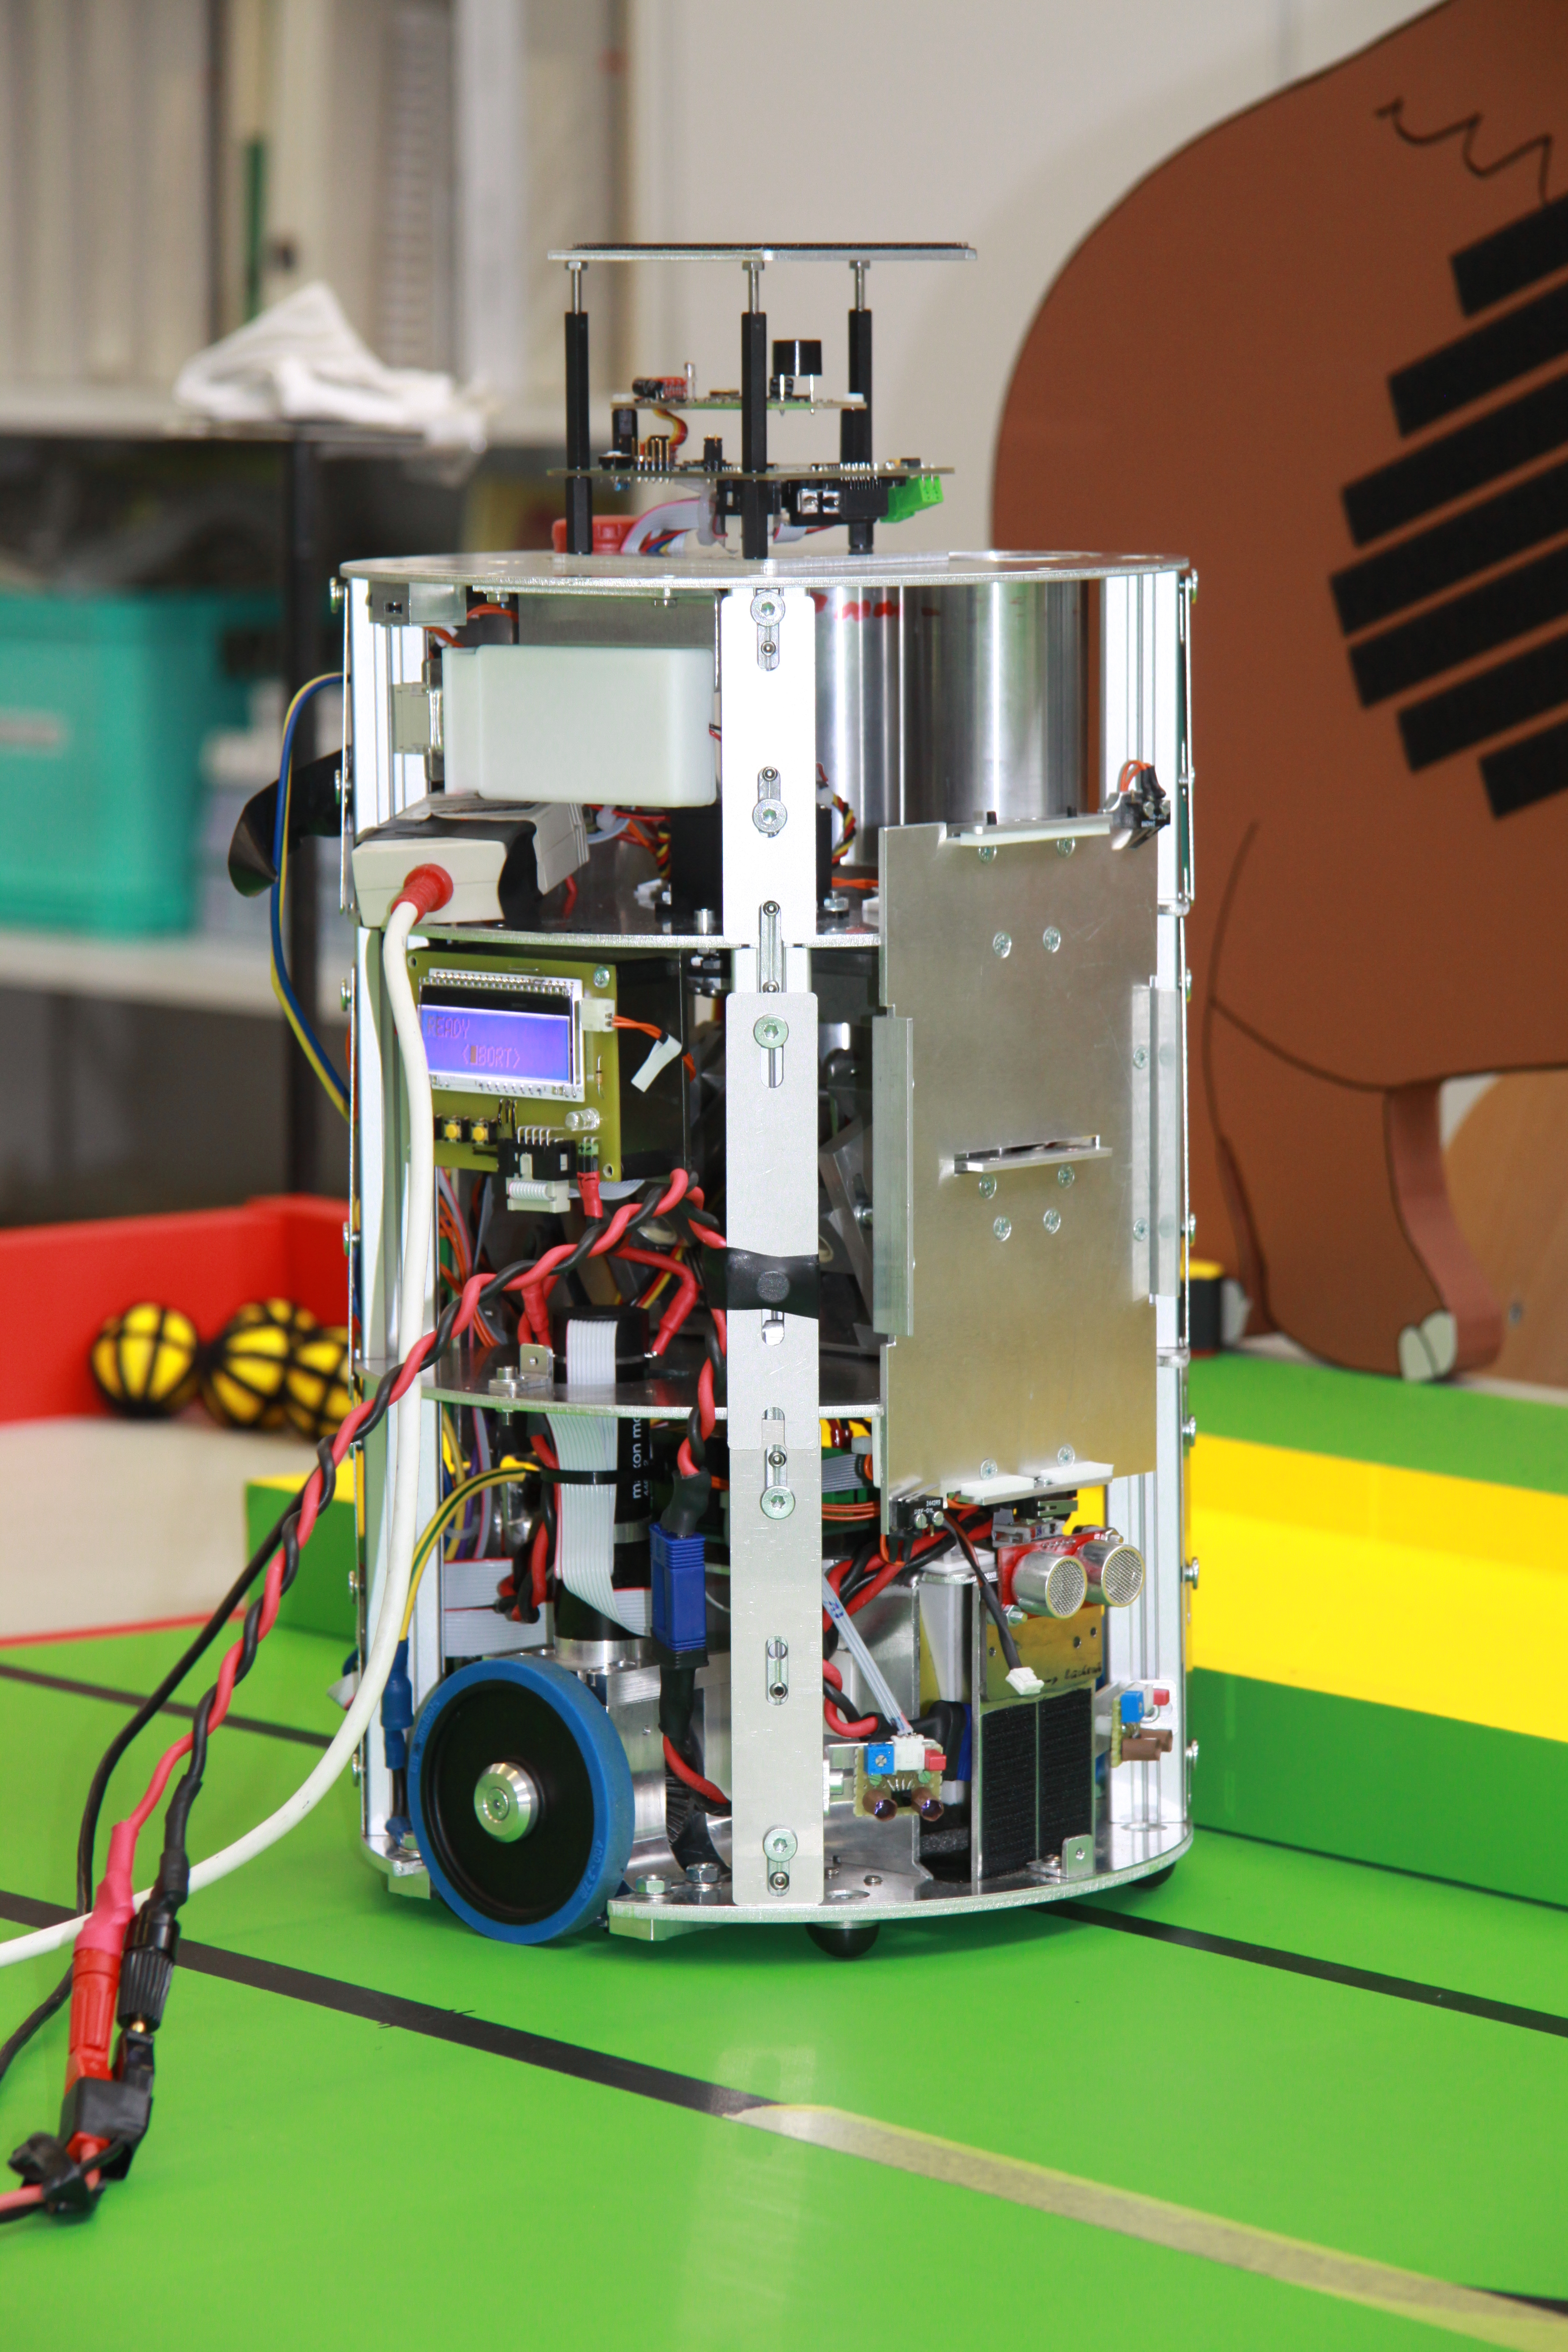
\includegraphics[height=8cm]{abstract/image/Roboter_klein}       
			\caption{"Ballerina"}
			\label{abb:robo_klein}
		\end{subfigure}
		\begin{subfigure}[b]{0.49\textwidth}
			\centering
			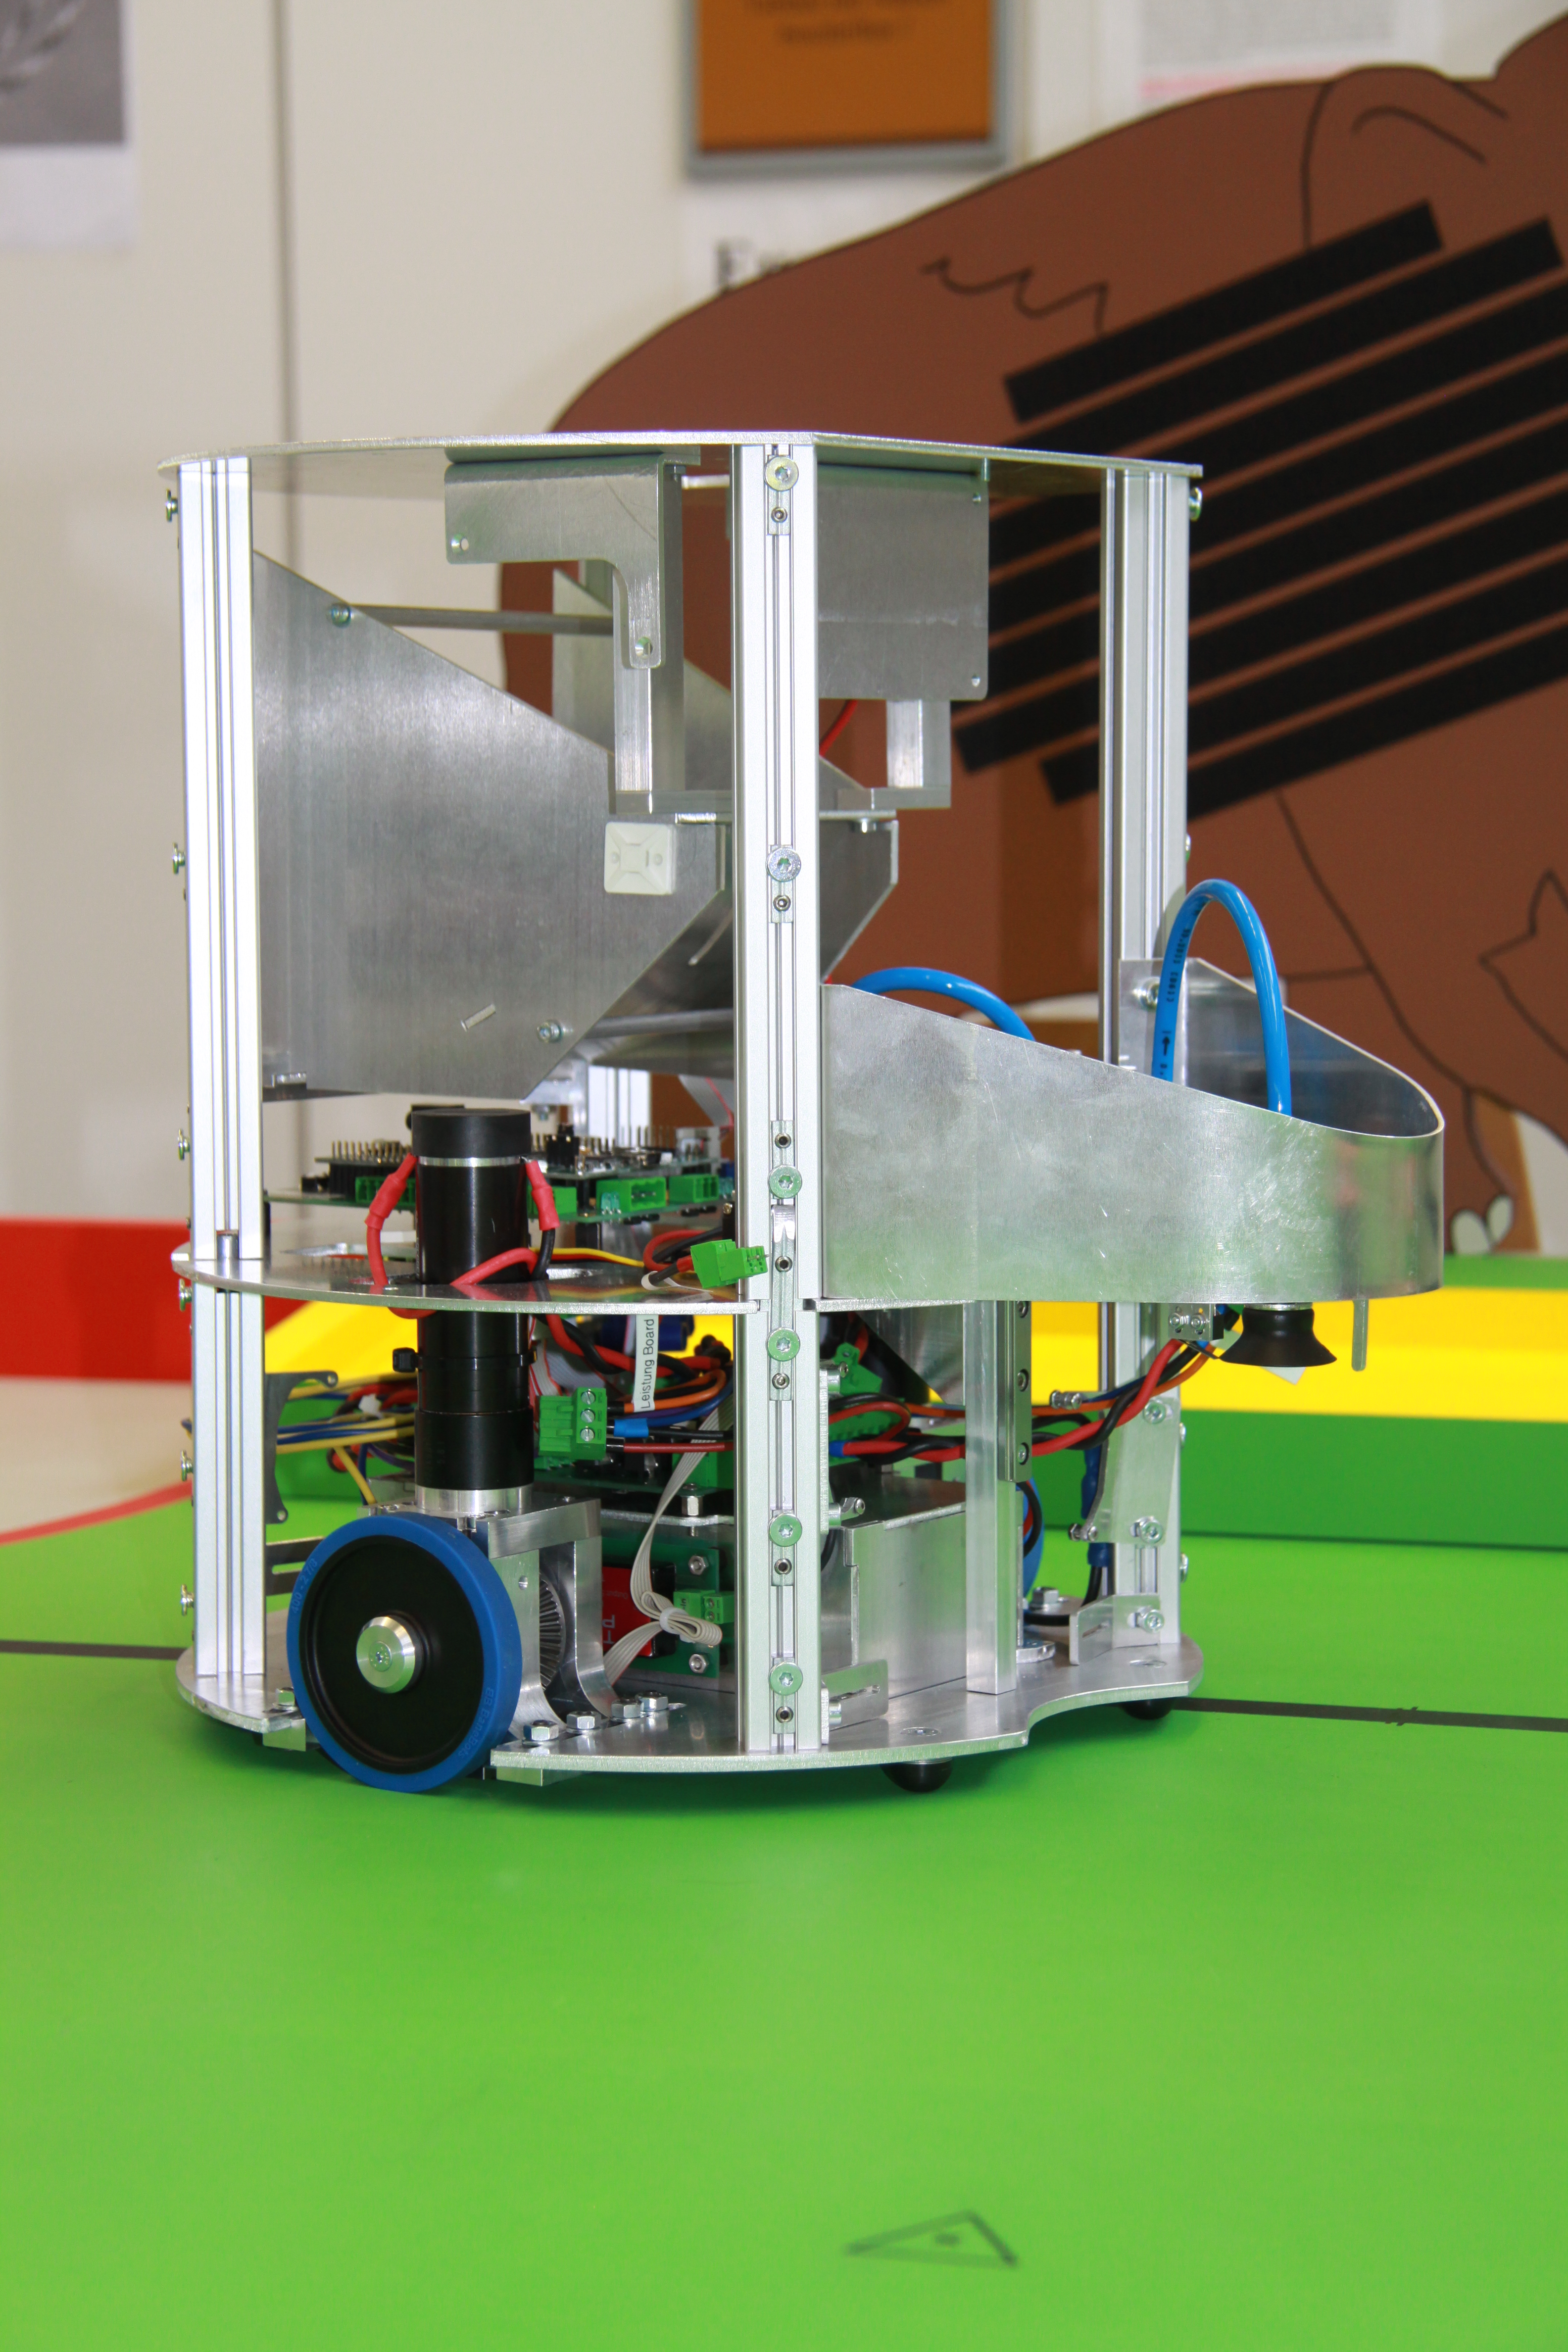
\includegraphics[height=8cm]{abstract/image/Roboter_gross}    
			\caption{"B52"}    
			\label{abb:robo_gross} 
		\end{subfigure}
		%\caption{Knoten ID's}
		%\label{abb:node_id}
   	\end{figure}